\documentclass[10pt,sigconf]{acmart}

\usepackage[utf8]{inputenc}
\usepackage{booktabs} % For formal tables
\usepackage{array}
\usepackage{commath}
\newcommand*\rotbf[1]{\rotatebox{90}{\textbf{#1}}}
\newcommand{\specialcell}[2][c]{\begin{tabular}[#1]{@{}l@{}}#2\end{tabular}}
\newcommand{\specialcellbold}[2][c]{%
  \bfseries
  \begin{tabular}[#1]{@{}l@{}}#2\end{tabular}%
}

% Copyright
%\setcopyright{none}
%\setcopyright{acmcopyright}
%\setcopyright{acmlicensed}
% \setcopyright{rightsretained}
%\setcopyright{usgov}
%\setcopyright{usgovmixed}
%\setcopyright{cagov}
%\setcopyright{cagovmixed}

\begin{document}
\title{Text Mining in Practice: Comment Volume Prediction}
\subtitle{Extended Abstract} % do we need that?

\author{Johannes M. Kroschewski}
\affiliation{%
	\institution{Hasso-Plattner-Institut,\\ University of Potsdam}
	\streetaddress{Prof.-Dr.-Helmert-Str. 2–3}
	\city{Potsdam} 
	\state{Germany} 
	\postcode{14482}
}
\email{johannes.kroschewski@student.hpi.de}

\author{Friedrich C. Schöne}
\affiliation{%
	\institution{Hasso-Plattner-Institut,\\ University of Potsdam}
	\streetaddress{Prof.-Dr.-Helmert-Str. 2–3}
	\city{Potsdam} 
	\state{Germany} 
	\postcode{14482}
}
\email{friedrich.schoene@student.hpi.de}

\author{Nils H. Straßenburg}
\affiliation{%
  	\institution{Hasso-Plattner-Institut,\\ University of Potsdam}
	\streetaddress{Prof.-Dr.-Helmert-Str. 2–3}
	\city{Potsdam} 
	\state{Germany} 
	\postcode{14482}
}
\email{nils.strassenburg@student.hpi.de}

% The default list of authors is too long for headers}
\renewcommand{\shortauthors}{M. Kroschewski et al.}


\begin{abstract}
	abstract text \footnote{abstract footnote}
\end{abstract}
%
% The code below should be generated by the tool at
% http://dl.acm.org/ccs.cfm
% Please copy and paste the code instead of the example below. 
%
\begin{CCSXML}
	% TODO
<ccs2012>
 <concept>
  <concept_id>10010520.10010553.10010562</concept_id>
  <concept_desc>Computer systems organization~Embedded systems</concept_desc>
  <concept_significance>500</concept_significance>
 </concept>
 <concept>
  <concept_id>10010520.10010575.10010755</concept_id>
  <concept_desc>Computer systems organization~Redundancy</concept_desc>
  <concept_significance>300</concept_significance>
 </concept>
 <concept>
  <concept_id>10010520.10010553.10010554</concept_id>
  <concept_desc>Computer systems organization~Robotics</concept_desc>
  <concept_significance>100</concept_significance>
 </concept>
 <concept>
  <concept_id>10003033.10003083.10003095</concept_id>
  <concept_desc>Networks~Network reliability</concept_desc>
  <concept_significance>100</concept_significance>
 </concept>
</ccs2012>  
\end{CCSXML}

\ccsdesc[500]{Computer systems organization~Embedded systems}
\ccsdesc[300]{Computer systems organization~Redundancy}
\ccsdesc{Computer systems organization~Robotics}
\ccsdesc[100]{Networks~Network reliability}

% We no longer use \terms command
%\terms{Theory}

\keywords{text mining}

\maketitle

\section{Introduction}
% \subsection{Motivation and Goal}

% \subsection{Related Work}


\section{Dataset}
Our work is based on a dataset taken from the British newspaper \textit{The Guardian} that contains approximately $626$K article URLs with $61.5$M corresponding comments from $1.25$M authors. 
The comment data provided us with the comment text itself, the author, the timestamp when the comment was posted, a reference of the parent comment, and the number of upvotes. Additionally, we had the comment author's username and a dedicated reference. 

The comments were posted between 2006 and 2017. All $1.25$M users wrote at least one comment, $22$\% of them more than $10$, and $6$\% over $100$.
The given articles are published in one out of $79$ categories. In total, $18$\% of all released articles are published under the category \textit{comment is free} which is used to debate contentious issues. Consequently, this category is also the most commented one. 
Each of the others, e.g. \textit{sport}, \textit{music}, and \textit{politics} covers less than $7$\% in the given dataset.

The number of comments of past articles is essential to predict the comment volume of similar articles in the future. 
To decide if a given article was in the top $10$\% of the most commented articles within its released week could be determined by simply counting the corresponding comments of each article.
%The number of comments of a given article is essential to predict the comment volume of similar articles in the future. Fortunately, this could be determined by simply counting the corresponding comments of each article. Afterwards, we were able to decide if a given article was in the top $10$\% of the most commented articles within its released week.

\subsection{Data Cleaning}
Analysing the dataset, we noticed that the distribution of the number of comments exhibited a bizarre peak at exactly $50$ comments per article. Therefore, we did not take these articles into account which reduced our dataset about $2$\% of the given articles.

To avoid anomalies using features that we derived from the articles, e.g. the publication time, we removed a small amount of articles that were released on 29th of February.

\subsection{Data Enrichment}
To enrich our dataset, we used the offical \textit{Guardian API} to get the article text and further attributes like the category, the headline, and the publication time.
Due to API restrictions we were not able to download all articles which is why the amount of articles was reduced about $11$\%.
Furthermore, we extracted metadata like the headline and article word count, the time data describing the day of the week, the day of the year, the hour and the minute of the publication date.

We suppose that articles that are released at a similar time and discussing a related topic are likely to share the amount of comments. To take this behaviour into account, we've developed a \textit{competitive score} (\ref{eq:competitive_score}) as an additional feature.

\begin{equation} \label{eq:competitive_score}
	compet_i = \sum_{n=1}^{j} \frac{\sigma'(t_i - t_j)}{\norm{\overrightarrow{a_i} - \overrightarrow{{a_j}}}^2}, i \neq j
\end{equation}

\begin{flalign*}
	\sigma&: \text{sigmoid function} & \\
	t_i&: \text{publication date of article } i & \\
	\overrightarrow{a_i}&: \text{doc2vec vector of article } i \text{ text}& \\
\end{flalign*}

The numerical value of $compet_i$ describes how much a given article $i$ competes with all other articles. Thereby, the difference of the publication time of the given articles determines how close they are published to each other. For the calculation of this feature, we've considered all articles that were released within a timespan of $\pm3$h.
In pratice, articles will be often published at the same time which implies that the time difference can be zero. This is also a reason why we apply the derivate of the sigmoid function in the numerator.
To decide if articles are discussing a similar topic, we've trained the \textit{doc2vec} algorithm \cite{le2014doc2vec} on our article corpus and use the Euclidean distance to calculate how similar articles to each other are. We square the distance in the denominator to increase the impact of the article similarity.

In the following, we call the cleaned and enriched dataset the Guardian Article and Comment Corpus (GACC). Finally, the GACC contains approximately $547$K articles with $58.6$M comments.


\section{Methodology}
To evaluate the quality of our features, different architectures were implemented to compare how accurately they predict comment volume.
All seven architectural models use single or related features as input and generate a binary classification output using sigmoid as the activation function. 
Each model has an identifier which will be used as a reference within the further text.

\subsection{Architectures}

\paragraph{Model 1} 
Takes the article headline as input.
The headline length is normalized before embedding the words using an embedding layer which is initialized with pretrained glove embeddings \cite{pennington2014glove}.
The model uses a dense and a batch normalization layer as the hidden layers.

\paragraph{Model 2}
Takes the article headline as input which is than embedded as in \textit{Model 1}. 
A convolutional layer with kernel sizes one, three, and five is used instead of a dense layer as well as a pooling layer as proposed by Kim \cite{kim2014convolutional}.

\paragraph{Model 3} 
Takes the first $50$ words of the article text which are embedded the same way as in \textit{Model 1} and \textit{2}. However, the input is processed through an LSTM layer outputting its last cell state.

\paragraph{Model 4} 
Takes the article category as input.
The category reference gets embedded using an embedding layer and is processed through both a dense and a batch normalization layer.

\paragraph{Model 5} 
Takes temporal features of the article's publication date as input.
The features are minute, hour, day of the week, and day of the year.
They get processed the same way as in \textit{Model 4}.

\paragraph{Model 6} 
Takes the word counts from the headline and the article.
The logarithm is calculated for both of them and is used to create exponential sized bins for different lengths.
Each logarithm gets embedded and processed as in \textit{Model 5} and \textit{6}.

\paragraph{Model 7} 
Takes the competitive score as defined in \autoref{eq:competitive_score} and processes it through a dense layer as well as a batch normalization layer.

\subsection{Training}
The GACC was divided into training, validation, and test sets using a $0.70/0.15/0.15$  distribution with respect to the time of publication.

Due to the strongly imbalanced class sizes of the training set, we use class weights to penalise our models in case of a wrong classification.
During the training, they influence the weighting of the loss indirectly proportional to the class size of a giving training sample.

\subsection{Combined Architectures}
We combined several models to explore how using multiple features simultaneously would impact our results.
These combined models share the classification layers but not the hidden layers.
Specific models were only combined if they performed adequately and if their results had some correlation.
Combining these two metrics, we had a large set of models we were able to choose from.
The correlations between each model pair are shown in Figure \ref{fig:correlation_matrix}. 

\begin{figure}[h]
	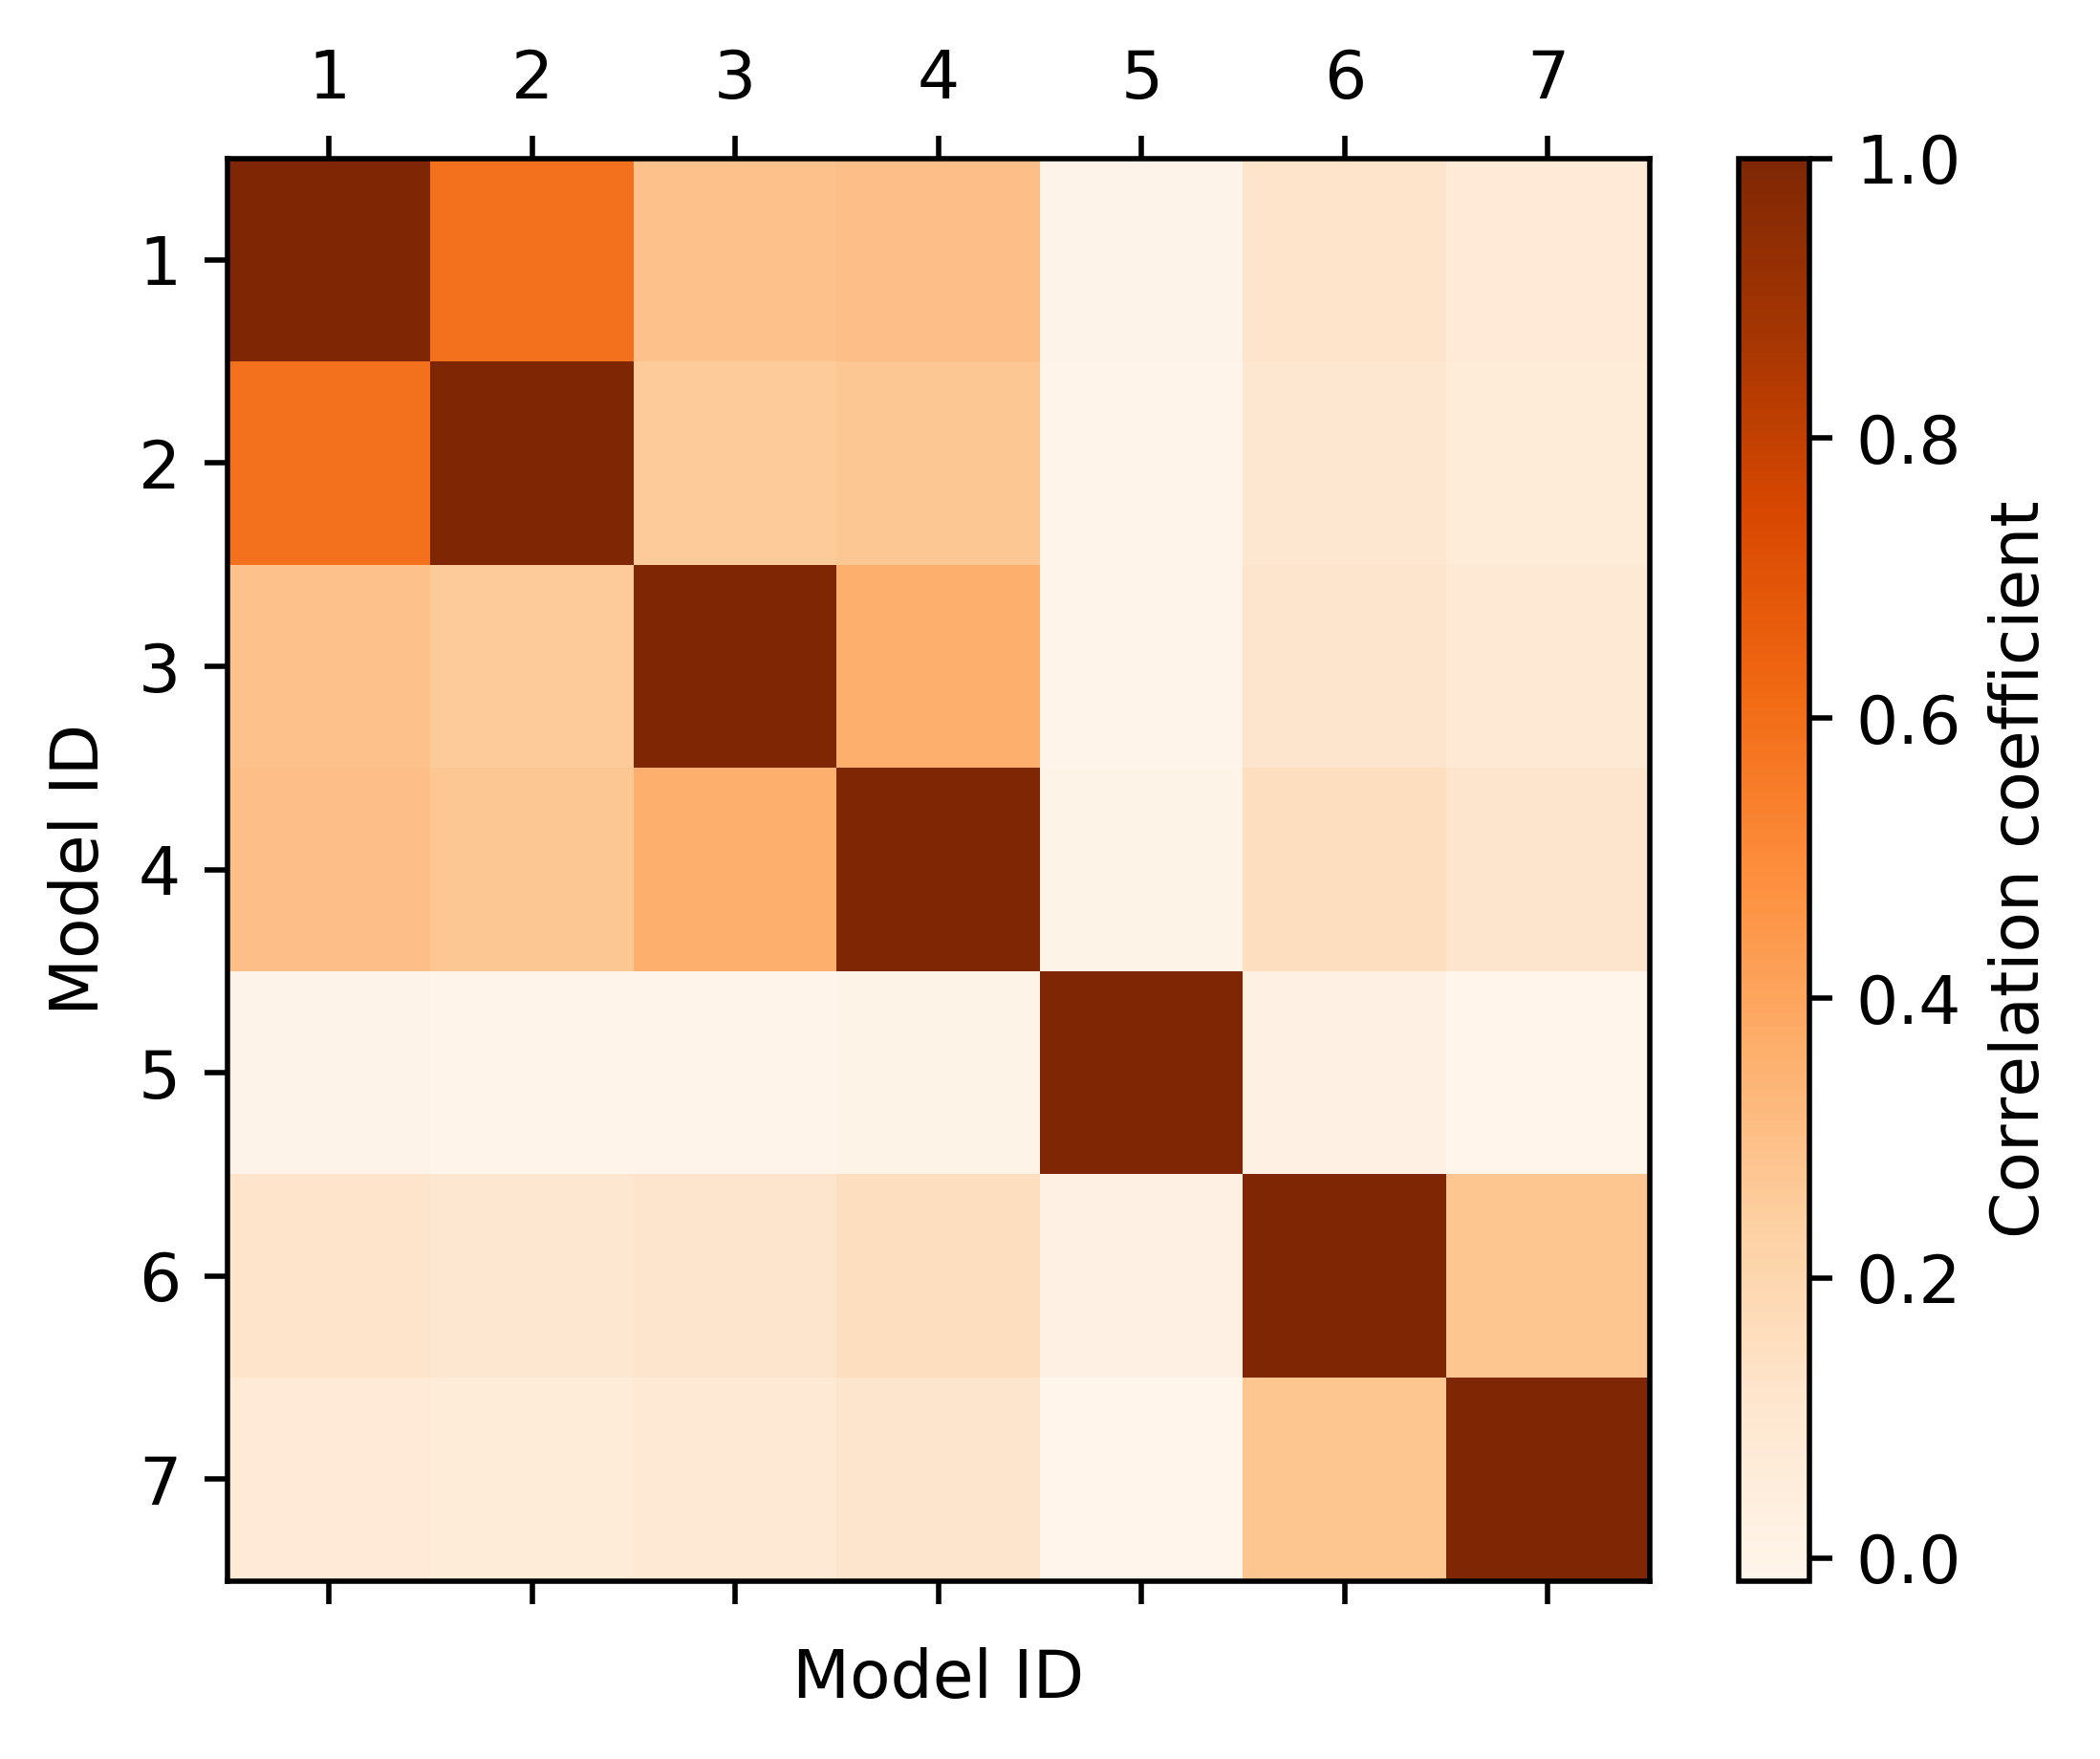
\includegraphics[width=0.3\textwidth]{fig/correlations.png}
	\caption{\textmd{Correlation matrix of our models using the test data set.}}
	\label{fig:correlation_matrix}
\end{figure}



\section{Evaluation}
% \begin{table}[]
% \centering
% \label{tbl:heatwheel_res}
% \begin{tabular}{cccccc}
% \toprule
% % \textbf{Features} &
% \specialcellbold{ID} &
% \specialcellbold{Input} &
% \specialcellbold{Model} &
% \specialcellbold{P} &
% \specialcellbold{R} &
% \specialcellbold{F1} \\
% \midrule
% 1 & headline & FC & .216 & .606  & .309  \\
% 2 & headline & CNN & .221 & .603  & .314  \\
% 3 & article & LSTM  & .228 & .493  & .302  \\
% 4 & category & FC & .227 & .603  & .320  \\
% 5 & time & FC  & .100 & .457  & .155  \\
% 6 & text metrics & FC  & .133 & .738  & .222  \\
% 7 & competitive score & FC & .112 & .917  & .197  \\
% \bottomrule
% \end{tabular}
% \end{table}
% \begin{table}[]
% \centering
% \label{tbl:heatwheel_res}
% \begin{tabular}{cccc}
% \toprule
% % \textbf{Features} &
% % \specialcellbold{Short description} &
% \specialcellbold{Combination} &
% \specialcellbold{P} &
% \specialcellbold{R} &
% \specialcellbold{F1} \\
% \midrule
% 2 3 & .224 & .645 & .323\\
% 2 4 & .245 & .627 & .342\\
% 2 5 & .227 & .581 & .317 \\
% 2 6 & .217 & .651 & .317\\
% 2 7 & .214 & .625 & .311\\
% 3 4 & .252 & .577 & .339\\
% 2 3 4 & .265 & .607 & .357\\
% \bottomrule
% \end{tabular}
% \end{table}

\subsection{Metrics}
% which metrics and why we used them
% cite other evaluation metrics

\subsection{Model Performances}
% explanation for good and bad performances

\subsection{Model Combinations}
% correlations and combination performances


\section{Conclusion}



\bibliographystyle{acm}
\bibliography{sigproc} 

\end{document}
